% !TEX ROOT = ../ersti.tex
% 
% TODO stefanzen
% 
% Nicht vergessen die Copyright Zeile im Impressum wieder einzufügen
% —done!

%\section{Semesterticket}
\mathphyssecnobar{Semesterticket}
Seit mehr als 15 Jahren hat Heidelberg ein Semesterticket, 
das es den Studierenden ermöglicht kostengünstig den öffentlichen
Nahverkehr zu nutzen.
Zur Einführung waren alle Beteiligten von der großen Resonanz überrascht
und das Ticket entwickelte sich zu einem Erfolg.
Enorme Preissteigerungen von 127\% in den vergangenen 10\,Jahren haben
jedoch dazu geführt, dass die Nutzerzahlen deutlich sinken und 
das Semesterticket von vielen als unattraktiv und überteuert wahrgenommen 
wird.

Ein Semesterticket muss stets eine Vielzahl von Interessen befriedigen. Es 
sollte ein attraktives und günstiges Ticket im Stadtbereich sein und das 
direkte Umfeld des Hochschulstandortes erschließen. Des Weiteren ist es wünschenswert die ländliche Region anzubinden und den dort wohnhaften Studierenden einen Umzug und hohe Mieten zu ersparen. Neben dem täglichen Pendelverkehr ist die Heimreise zum elterlichen Wohnsitz ebenfalls für eine Vielzahl von Studierenden ein Grund ein Semesterticket zu erwerben.

Das aktuelle Semesterticket in Heidelberg wird vom Verkehrsverbund Rhein-Neckar (VRN) angeboten und gilt für ein Semester. Es berechtigt zu Fahrten im gesamten Tarifgebiet\footnote{\url{http://www.vrn.de/linienplaene/netzlinienplaene/gesamtnetz/}} -- „einem Schlauch von Polen nach Frankreich“\footnote{Zitat aus der Semesterticket Umfrage der FSK}. Die Ausdehnung ist in Ost-West Richtung sehr weitreichend, in Nord-Süd Richtung ist jedoch nach 20\,km von Heidelberg aus Schluss. Das Semesterticket finanziert sich aus einem Kaufpreis von aktuell \EUR{150} und einem solidarischen Sockelbeitrag von \EUR{25.80}, den alle Studierenden mit dem Studentenwerksbeitrag bei der Rückmeldung zahlen müssen -- auch wenn sie das Ticket nicht nutzen. Eine Heidelberger Besonderheit bei der Sockelfinanzierung ist, dass sie es allen Studierenden ermöglicht ab 19 Uhr innerhalb der Großwabe Heidelberg sowie den Waben Dossenheim, Eppelheim und Leimen kostenlos mit Bus und Bahn fahren zu können -- der Studiausweis gilt dabei als Fahrschein.


\subsection{Konflikt ums Semesterticket}
\marginpar{
    \centering
    \vspace{1mm}
    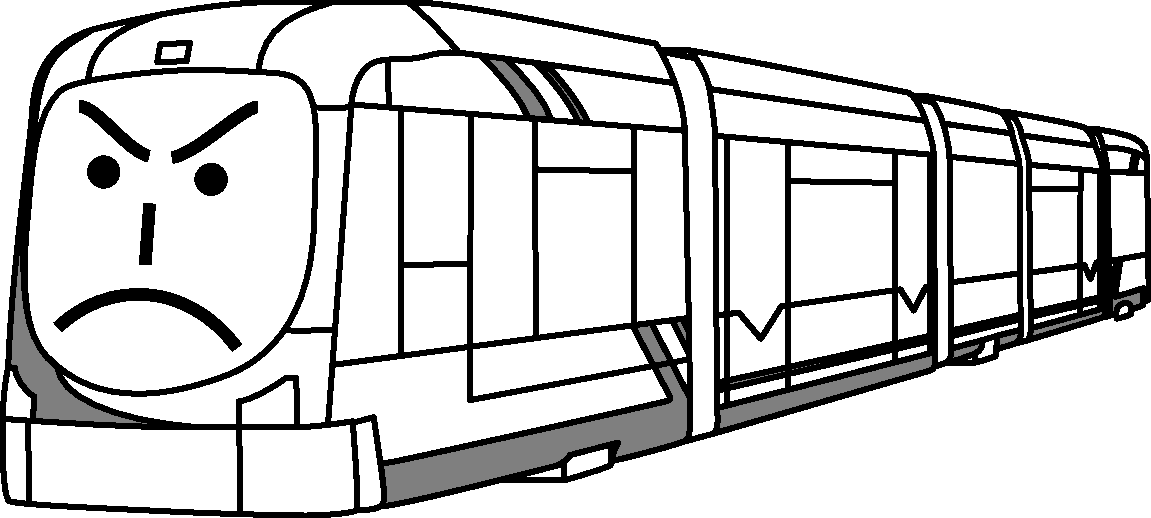
\includegraphics[width=3cm]{bilder/straba.pdf}
}
Seit Herbst 2008 verhandeln das Verkehrsreferat der Studierendenvertretung und das Studentenwerk mit dem VRN über einen neuen Vertrag. Die Studis fordern ein Ende der enormen Preissteigerungen, um auch in Zukunft mit dem Semesterticket ein günstiges Nahverkehrsangebot zu gewährleisten. Da der VRN jedoch weiter an Preissteigerungen von ca. 10\% pro Jahr festhalten will, stand das Semesterticket vor dem Aus. 
Nach einem Übergangsvertrag, auf den der VRN sich im WS 09/10 in letzer Minute eingelassen hat, wurde im WS 13/14 erneut verhandelt. Diesmal kam der Kommunalwahlkampf in Heidelberg den Studis zu Gute, aber trotz massiven Drucks aus der Politik und Zuschüssen durch den Gemeinderat ist das Semesterticket nach wie vor recht teuer und der VRN wird die Preise weiterhin regelmäßig erhöhen.

Eine Neuerung bei den letzten Vertragsverhandlungen war, dass der frisch eingerichtete \gls{StuRa} alle Studis zu einer Urabstimmung über das Vertragsangebot aufgerufen hat. Auch wenn die Urabstimmung wegen teils schwerer Formfehler von verschiedenen Seiten angefochten wurde, hat sich doch eine Mehrheit der Abstimmenden für das Semesterticket ausgesprochen, sodass der StuRa dem Vertragsangebot letztendlich zugestimmt hat.\\[1em]

Heidelberg ist eine eher kleine übersichtliche Stadt in welcher alles bequem mit dem Fahrrad erledigt werden können -- meist sogar schneller als mit Bus und Bahn. Dank der milden Temperaturen ist dies auch im Winter durchaus möglich. Wenn ihr in Heidelberg selbst wohnt ist daher gut zu überlegen ob sich ein Semesterticket lohnt oder man wie viele Andere das Fahrrad nutzt.

Weitere Informationen zu den Verhandlungen und dem Semesterticket findest du unter: \url{http://www.stura.uni-heidelberg.de/semesterticket}

%~ \begin{figure}[h]
%~ \centering{
    %~ 
\includegraphics[width=\textwidth]{bilder/purity.png}
%~ }
%~ \end{figure}


